\chapter{Fourth Requirement}
\section{Decompressing Image using IDCT}
To get the original image we decompress the compressed image using IDCT but on the retained $m$x$m$ block with ignoring the other values by setting them to zeros.

\begin{tcolorbox}[colback=green!8!white,colframe=green!40!black,title=\textbf{Inverse Discrete Cosines Transform}]
    $$x\left[m,n\right] =  \sum_{p=0}^{M-1}\sum_{q=0}^{N-1}\alpha_p \alpha_q X[p,q] \cos{\frac{\pi \left(2m+1\right)p}{2M}} \, \cos{\frac{\pi \left(2n+1\right)q}{2N}}$$
    $$\alpha_p = \begin{cases}
        \frac{1}{\sqrt{M}}\hspace{27pt} p=0 \\\\
        \sqrt{\frac{2}{M}}\,\,\, 1 \leq p \leq M - 1
    \end{cases}
    \alpha_q = \begin{cases}
        \frac{1}{\sqrt{N}}\hspace{27pt} q=0 \\\\
        \sqrt{\frac{2}{N}}\,\,\, 1 \leq q \leq N - 1
    \end{cases}
    $$
\end{tcolorbox}
\vspace{5pt}
\lstinputlisting[language=Python,caption={Code For Decompressing The Compressed Image.}]{DecompressingImage.py}
\noindent We will show below how increasing m can effectively change the quality of the image.

\begin{figure}[h]
    \centering
    
\includegraphics[width=0.9\textwidth]{../Decompressed Images/decompressedImage_m1.png}
    \caption{Decompressed image using $m=1$.}
    \label{fig:decompressed_img_m1}
\end{figure}

\begin{figure}[h]
    \centering
    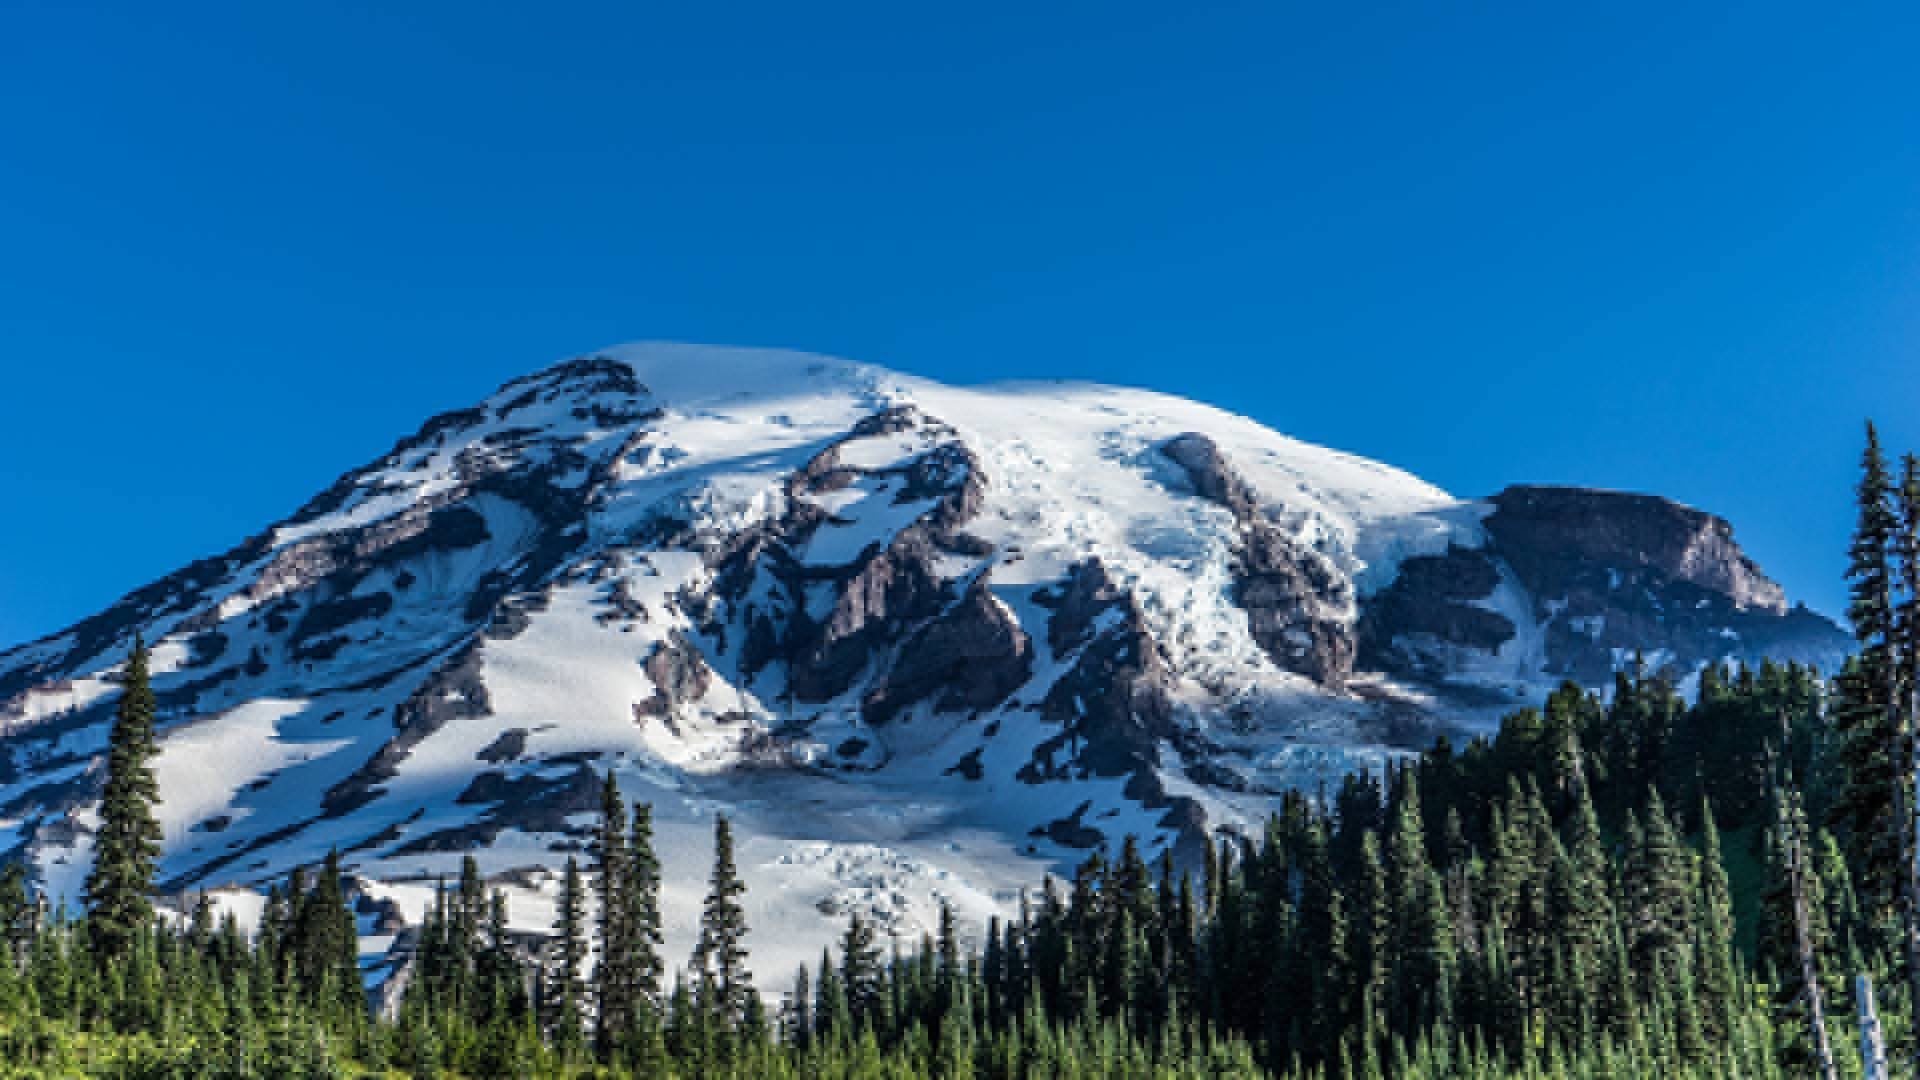
\includegraphics[width=0.9\textwidth]{../Decompressed Images/decompressedImage_m2.png}
    \caption{Decompressed image using $m=2$.}
    \label{fig:decompressed_img_m2}
\end{figure}

\begin{figure}[h]
    \centering
    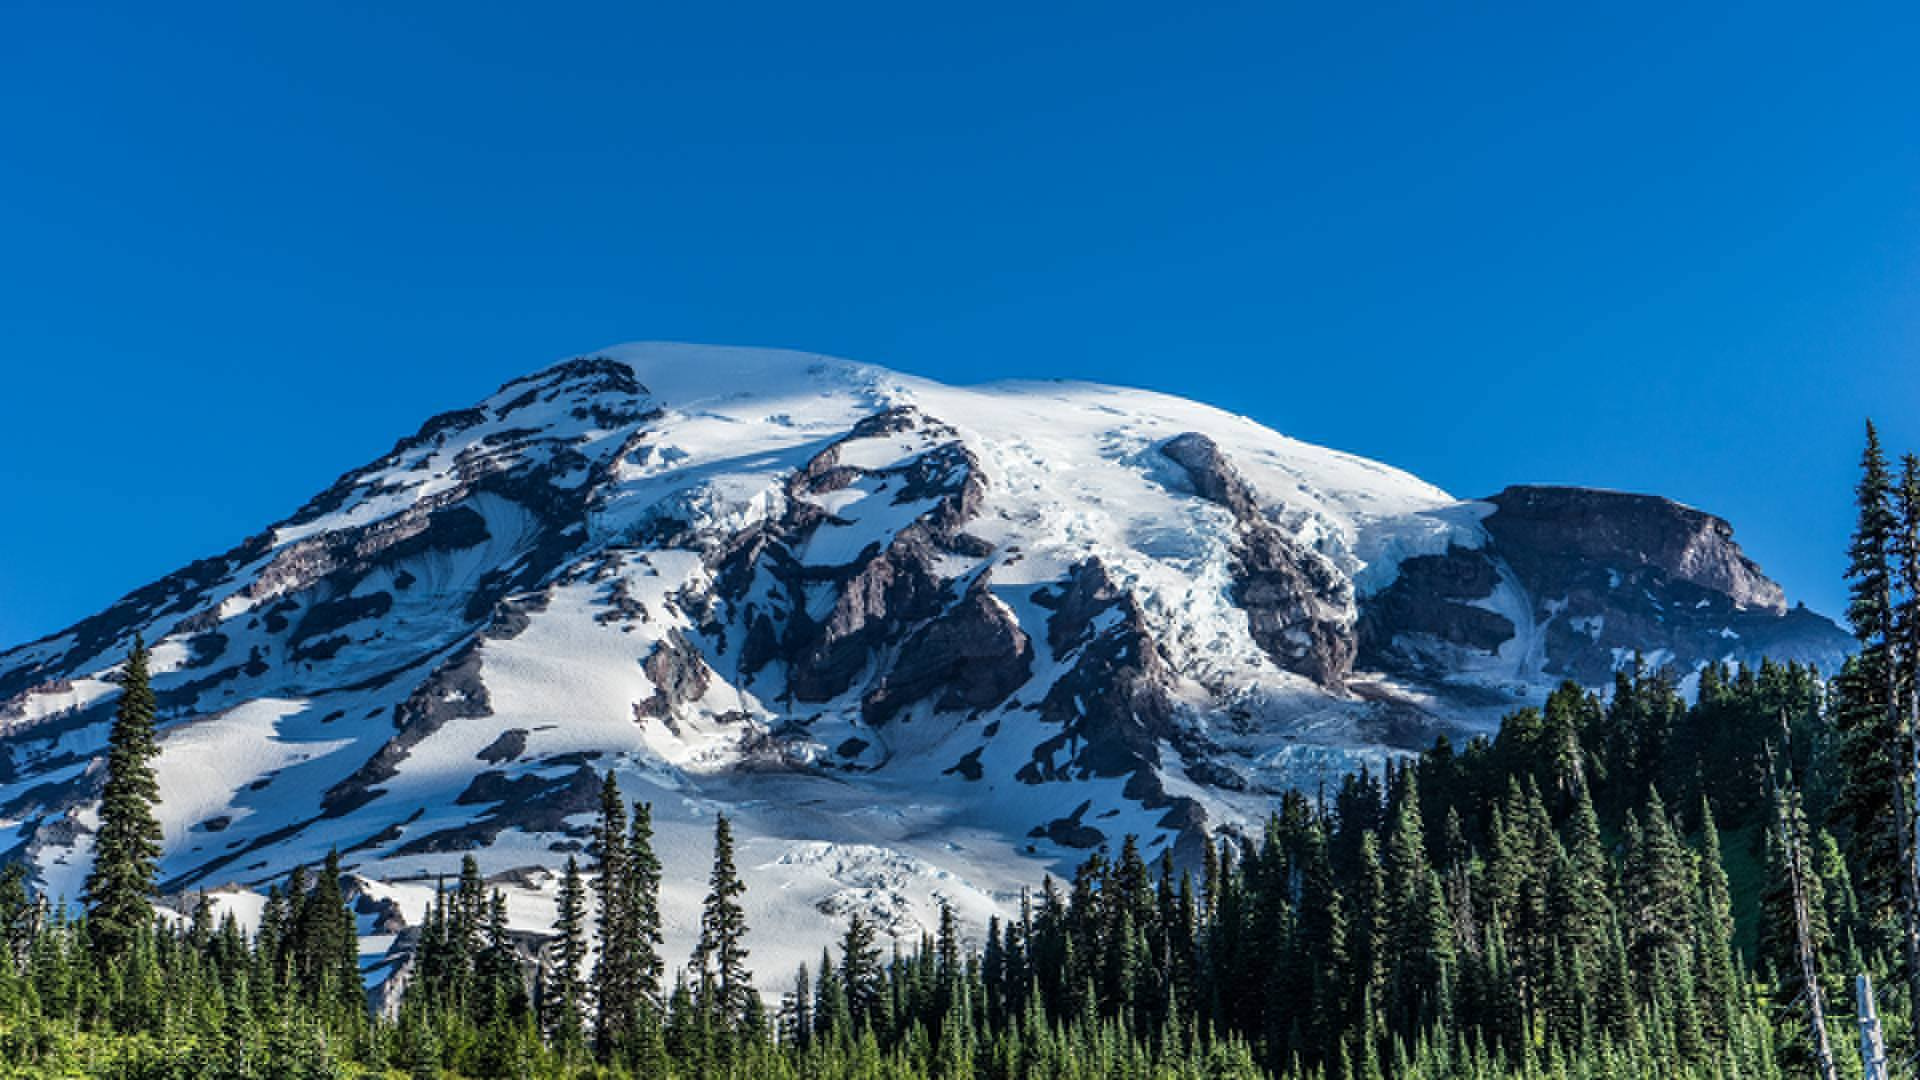
\includegraphics[width=0.9\textwidth]{../Decompressed Images/decompressedImage_m3.png}
    \caption{Decompressed image using $m=3$.}
    \label{fig:decompressed_img_m3}
\end{figure}

\begin{figure}[h]
    \centering
    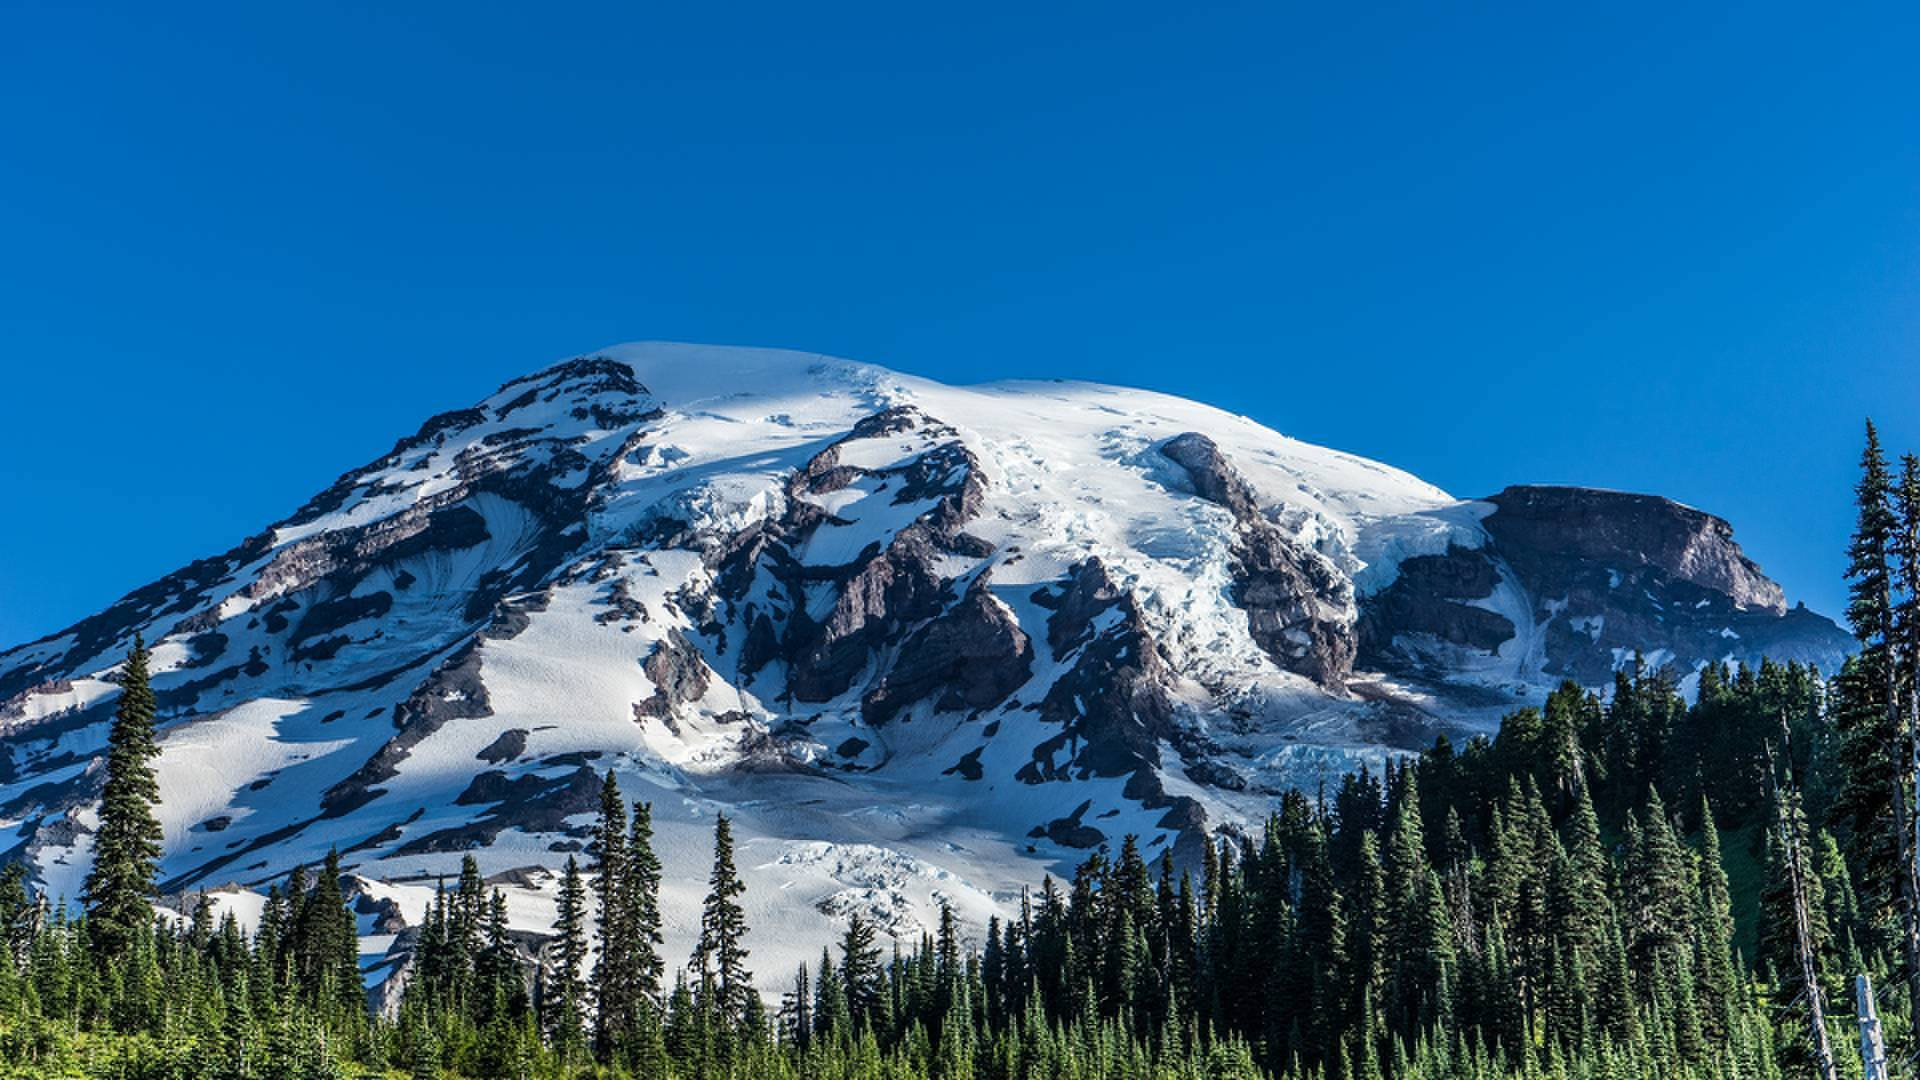
\includegraphics[width=0.9\textwidth]{../Decompressed Images/decompressedImage_m4.png}
    \caption{Decompressed image using $m=4$.}
    \label{fig:decompressed_img_m4}
\end{figure}

